\documentclass[tikz]{standalone}
\usepackage{tikz}
\usetikzlibrary{patterns,snakes,angles}
 
\begin{document}
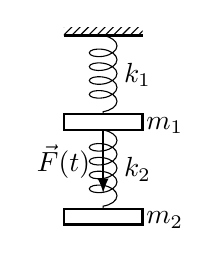
\begin{tikzpicture}
	\draw [draw=none, pattern=north east lines] (-0.5,0) rectangle (0.5,0.1);
	\draw [thick] (-0.5,0) -- (0.5,0);
	\draw [snake=coil, segment amplitude=5pt, segment length=5pt] (0,0) -- (0,-1) node [midway, right=4pt] {$k_1$};
	\draw [snake=coil, segment amplitude=5pt, segment length=5pt] (0,-1.2)-- (0,-2.2) node [midway, right =4pt] {$k_2$};
	\draw [thick] (-0.5,-1) rectangle (0.5, -1.2) node [right=8pt, above=-5pt] {$m_1$};
	\draw [thick] (-0.5,-2.2) rectangle (0.5, -2.4) node [right=8pt, above=-5pt] {$m_2$};
	\draw [thick, arrows={-latex}] (0,-1.2) -- (0,-2.0) node [midway, left=1pt] {$\vec{F}(t)$};
\end{tikzpicture}
\end{document}